%%%%%%%%%%%%%%%%%%%%%%%%%%%%%%%%%%%%%%%
% Programming/Coding Assignment
% LaTeX Template
%
% This template has been downloaded from:
% http://www.latextemplates.com
%
% Original author:
% Ted Pavlic (http://www.tedpavlic.com)
%
% Note:
% The \lipsum[#] commands throughout this template generate dummy text
% to fill the template out. These commands should all be removed when 
% writing assignment content.
%
% This template uses a Perl script as an example snippet of code, most other
% languages are also usable. Configure them in the "CODE INCLUSION 
% CONFIGURATION" section.
%
%%%%%%%%%%%%%%%%%%%%%%%%%%%%%%%%%%%%%%%%%

%----------------------------------------------------------------------------------------
%	PACKAGES AND OTHER DOCUMENT CONFIGURATIONS
%----------------------------------------------------------------------------------------

\documentclass[a4paper]{article}

\usepackage{fancyhdr} % Required for custom headers
\usepackage{lastpage} % Required to determine the last page for the footer
\usepackage{extramarks} % Required for headers and footers
\usepackage[usenames,dvipsnames]{color} % Required for custom colors
\usepackage{graphicx} % Required to insert images
\usepackage{listings} % Required for insertion of code
\renewcommand*{\lstlistingname}{代码} % change "Listing <ref> to 代码 <ref>
\usepackage{courier} % Required for the courier font
\usepackage{lipsum} % Used for inserting dummy 'Lorem ipsum' text into the template

\usepackage[UTF8]{ctex} % Required for Chinese character
\usepackage{tocloft} % Required for beautiful toc
\usepackage[colorlinks]{hyperref} % Required for clickable toc
\hypersetup{
    colorlinks=false,
    citecolor=red,
    filecolor=black,
    linkcolor=blue,
    urlcolor=black,
    linkbordercolor	= {1 0 0}
}
\usepackage[title]{appendix} % Required for appendix
\usepackage{float}
\usepackage{amsmath} % used for \text{} in math formula


% used for beautiful table
\usepackage{booktabs} 
\usepackage[T1]{fontenc}
\usepackage{tabu}
\usepackage{longtable}
\usepackage[table]{xcolor}

\usepackage{algpseudocode}
\usepackage{algorithm}

%used for beautiful order list
\usepackage{enumitem}

\def\equationautorefname{式}%
\def\footnoteautorefname{脚注}%
\def\itemautorefname{项}%
\def\figureautorefname{图}%
\def\tableautorefname{表}%
\def\partautorefname{篇}%
\def\appendixautorefname{附录}%
\def\chapterautorefname{章}%
\def\sectionautorefname{节}%
\def\subsectionautorefname{小节}%
\def\subsubsectionautorefname{subsubsection}%
\def\paragraphautorefname{段落}%
\def\subparagraphautorefname{子段落}%
\def\FancyVerbLineautorefname{行}%
\def\theoremautorefname{定理}%
\def\algorithmautorefname{算法}
\let\subsubsectionautorefname\sectionautorefname

% TODO:
\newcommand{\aref}[1]{\hyperref[#1]{附录~\ref{#1}}}

% Margins
\topmargin=-0.45in
\evensidemargin=0in
\oddsidemargin=0in
\textwidth=6.5in
\textheight=9.0in
\headsep=0.25in

\linespread{1.1} % Line spacing

% Set up the header and footer
\pagestyle{fancy}
\lhead{\hmwkAuthorName} % Top left header
\chead{\hmwkClass\ (\hmwkClassInstructor\ \hmwkClassTime): \hmwkTitle} % Top center head
\rhead{\firstxmark} % Top right header
\lfoot{\lastxmark} % Bottom left footer
\cfoot{} % Bottom center footer
\rfoot{Page\ \thepage\ of\ \protect\pageref*{LastPage}} % Bottom right footer
\renewcommand\headrulewidth{0.4pt} % Size of the header rule
\renewcommand\footrulewidth{0.4pt} % Size of the footer rule

\setlength\parindent{0pt} % Removes all indentation from paragraphs

%----------------------------------------------------------------------------------------
%	CODE INCLUSION CONFIGURATION
%----------------------------------------------------------------------------------------

\definecolor{MyDarkGreen}{rgb}{0.0,0.4,0.0} % This is the color used for comments
% \lstloadlanguages{c} % Load Perl syntax for listings, for a list of other languages supported see: ftp://ftp.tex.ac.uk/tex-archive/macros/latex/contrib/listings/listings.pdf
% \lstset{language=sql, % Use Perl in this example
%         frame=single, % Single frame around code
%         basicstyle=\small\ttfamily, % Use small true type font
%         keywordstyle=[1]\color{Blue}, % Perl functions bold and blue
%         keywordstyle=[2]\color{Purple}, % Perl function arguments purple
%         keywordstyle=[3]\color{Blue}\underbar, % Custom functions underlined and blue
%         identifierstyle=, % Nothing special about identifiers                                         
%         commentstyle=\usefont{T1}{pcr}{m}{sl}\color{MyDarkGreen}\small, % Comments small dark green courier font
%         stringstyle=\color{Purple}, % Strings are purple
%         showstringspaces=false, % Don't put marks in string spaces
%         tabsize=4, % 5 spaces per tab
%         %
%         % Put standard Perl functions not included in the default language here
%         % morekeywords={rand},
%         morekeywords={rand, go},
%         %
%         % Put Perl function parameters here
%         morekeywords=[2]{REAL},
%         %
%         % Put user defined functions here
%         morekeywords=[3]{},
%        	%
%         morecomment=[l][\color{Blue}]{...}, % Line continuation (...) like blue comment
%         numbers=left, % Line numbers on left
%         firstnumber=1, % Line numbers start with line 1
%         numberstyle=\tiny\color{Blue}, % Line numbers are blue and small
%         stepnumber=2, % Line numbers go in steps of 5,
%         firstnumber=1
% }

\lstloadlanguages{C++}
\lstdefinestyle{mycpp}{
    language=C++, % Use Perl in this example
    frame=single, % Single frame around code
    basicstyle=\small\ttfamily, % Use small true type font
    keywordstyle=[1]\color{Blue}, % Perl functions bold and blue
    keywordstyle=[2]\color{Purple}, % Perl function arguments purple
    keywordstyle=[3]\color{Blue}\underbar, % Custom functions underlined and blue
    keywordstyle=[4]\color{Aquamarine}, % Custom functions underlined and blue
    identifierstyle=, % Nothing special about identifiers                                         
    commentstyle=\usefont{T1}{pcr}{m}{sl}\color{MyDarkGreen}\small, % Comments small dark green courier font
    stringstyle=\color{Purple}, % Strings are purple
    showstringspaces=false, % Don't put marks in string spaces
    tabsize=4, % 5 spaces per tab
    %
    % Put standard Perl functions not included in the default language here
    % morekeywords={rand},
    morekeywords={go, REFERENCES, DATABASE, SCHEMA},
    %
    % Put Perl function parameters here
    morekeywords=[4]{np},
    %
    % Put user defined functions here
    morekeywords=[1]{self},
    morekeywords=[3]{},
    %
    morecomment=[l][\color{Blue}]{...}, % Line continuation (...) like blue comment
    numbers=left, % Line numbers on left
    firstnumber=1, % Line numbers start with line 1
    numberstyle=\tiny\color{Blue}, % Line numbers are blue and small
    stepnumber=2, % Line numbers go in steps of 5,
    firstnumber=1
}
% Creates a new command to include a perl script, the first parameter is the filename of the script (without .pl), the second parameter is the caption

\newcommand{\shfilescript}[3]{
\begin{itemize}
\item[]\lstinputlisting[caption=#2, label=lst:#1, language=sh]{#3}
\end{itemize}
}
\newcommand{\shscript}[3]{
\begin{itemize}
\item[]\begin{lstlisting}[label=lst:#1, caption=#2] #3 \end{lstlisting}
\end{itemize}
}

%----------------------------------------------------------------------------------------
%	DOCUMENT STRUCTURE COMMANDS
%	Skip this unless you know what you're doing
%----------------------------------------------------------------------------------------

% Header and footer for when a page split occurs within a problem environment
\newcommand{\enterProblemHeader}[1]{
\nobreak\extramarks{#1}{#1 见下页\ldots}\nobreak{} 
\nobreak\extramarks{接上页}{#1 见下页\ldots}\nobreak{}
}

% Header and footer for when a page split occurs between problem environments
\newcommand{\exitProblemHeader}[1]{
\nobreak\extramarks{接上页}{#1 见下页\ldots}\nobreak{}
\nobreak\extramarks{#1}{}\nobreak{}
}
% TODO:code here enable the number before section, but it disable the numbering of problems
%\setcounter{secnumdepth}{0} % Removes default section numbers
\newcounter{homeworkProblemCounter} % Creates a counter to keep track of the number of problems

\newcommand{\homeworkProblemName}{}
\newenvironment{homeworkProblem}[1][Problem \arabic{homeworkProblemCounter}]{ % Makes a new environment called homeworkProblem which takes 1 argument (custom name) but the default is "Problem #"
\stepcounter{homeworkProblemCounter} % Increase counter for number of problems
\renewcommand{\homeworkProblemName}{#1} % Assign \homeworkProblemName the name of the problem
\section{\homeworkProblemName} % Make a section in the document with the custom problem count
\enterProblemHeader{\homeworkProblemName} % Header and footer within the environment
}{
\exitProblemHeader{\homeworkProblemName} % Header and footer after the environment
}

\newcommand{\problemAnswer}[1]{ % Defines the problem answer command with the content as the only argument
\noindent\framebox[\columnwidth][c]{\begin{minipage}{0.98\columnwidth}#1\end{minipage}} % Makes the box around the problem answer and puts the content inside
}

\newcommand{\homeworkSectionName}{}
\newenvironment{homeworkSection}[1]{ % New environment for sections within homework problems, takes 1 argument - the name of the section
\renewcommand{\homeworkSectionName}{#1} % Assign \homeworkSectionName to the name of the section from the environment argument
\subsection{\homeworkSectionName} % Make a subsection with the custom name of the subsection
\enterProblemHeader{\homeworkProblemName\ [\homeworkSectionName]} % Header and footer within the environment
}{
\enterProblemHeader{\homeworkProblemName} % Header and footer after the environment
}


\newcommand{\codev}[1]{\textsf{#1}}
%----------------------------------------------------------------------------------------
%	NAME AND CLASS SECTION
%----------------------------------------------------------------------------------------

% table color
\definecolor{tableHeader}{RGB}{245, 245, 245}
\definecolor{tableLineOne}{RGB}{245, 245, 245}
\definecolor{tableLineTwo}{RGB}{224, 224, 224}
\newcommand{\tableHeaderStyle}{
    \rowfont{\leavevmode\color{white}\bfseries}
    \rowcolor{tableHeader}
}

%----------------------------------------------------------------------------------------

\newcommand{\hmwkTitle}{人工智能\ \#博弈树搜索} % Assignment title
\newcommand{\hmwkDueDate}{Tuesday,\ December\ 27,\ 2018} % Due date
\newcommand{\hmwkClass}{16级计科\ 7班} % Course/class
\newcommand{\hmwkClassTime}{周三3-4节} % Class/lecture time
\newcommand{\hmwkClassInstructor}{饶洋辉} % Teacher/lecturer
\newcommand{\hmwkAuthorName}{颜彬} % Your name
\newcommand{\hmwkAuthorId}{16337269} % Your id 

%----------------------------------------------------------------------------------------
%	TITLE PAGE
%----------------------------------------------------------------------------------------

\usepackage{titling}

\title{
\vspace{2in}
\textmd{\textbf{\hmwkClass:\ \hmwkTitle}}\\
\normalsize\vspace{0.1in}\small{Due\ on\ \hmwkDueDate}\\
\vspace{0.1in}\large{\textit{\hmwkClassInstructor\ \hmwkClassTime}}
\vspace{3in}
}

\author{\textbf{\LARGE{\hmwkAuthorName}} \\ \\ \textbf{\LARGE{\hmwkAuthorId}}}
\date{} % Insert date here if you want it to appear below your name
%----------------------------------------------------------------------------------------

\begin{document}
% \begin{titlingpage} % This is for ignore page number in first page. package titling

\maketitle

%----------------------------------------------------------------------------------------
%	TABLE OF CONTENTS
%----------------------------------------------------------------------------------------

% \setcounter{tocdepth}{2} % Uncomment this line if you don't want subsections listed in the ToC
% set depth in toc

% \renewcommand{\cftsecleader}{\cftdotfill{\cftdotsep}} % used for dots between <section> and <page>

\renewcommand{\contentsname}{Content} % force the word to be "content
\newpage
\tableofcontents
\addtocontents{toc}{~\hfill\textbf{Page}\par}
\newpage

% below are document body


% To have just one problem per page, simply put a \clearpage after each problem
\section{算法简介}
\subsubsection{Minimax搜索}
Minimax算法即最大最小值算法,它是一种树型的搜索算法,被广泛运用在博弈类
问题上。\\

加深玩家与AI进行博弈(AI先手)。AI可能有多种行动方法,对每种行动玩家也有对应
的多种行动方法。Minimax搜索解决的问题是,如何为AI选择一种最适宜于当前局势的
行动方法。\\

Minimax算法的思路是,
\begin{itemize}
    \item 每当AI行动时,它总是会选择让AI胜率最高的方法行动
    \item 每当玩家进行行动时,他总是会选择让AI胜率最低的方法行动
\end{itemize}
当搜索树的某层
是轮到AI行动时,该层的结点的评分数会等于所有子结点评分的最大值,对玩家亦然。
运用这个算法搜遍整个博弈树(或搜索完某个特定深度),AI即可选出最佳的行动方法。\\

这就是算法名字的来历,他会交替地使用最大值和最小值来确定当前结点的估值。
如果当前结点的值由子节点的最大值来确定,那么当前结点称为最大结点,反之依然。\\

理论上,当整棵搜索树可以被完全遍历时,可以找到一个全局最优的下法。但搜索树往往
很大,无法被完全遍历。故一般搜索时会设定一个最大深度,当搜索达到深度上限时,
使用估值函数近似当前棋盘的局势。
\subsubsection{Alpha-beta剪枝}
Alpha-beta剪枝是一种minimax算法的剪枝方法。它的思路是,当搜索到的某个结点
的子结点评分太高或太低时,该结点很可能对整棵博弈树的评分没有影响(因为父结点很可能
根本不会犯傻走这个结点),于是进行剪枝,避免进行不必要的运算。\\

具体地说,在整个minimax的搜索中,维护两个变量$\alpha$(初始化为
$-\infty$)和$\beta$(初始化为$\infty$)。区间$[\alpha, \beta]$(初始
为$[-\infty, \infty]$)代表着一个``可接受的区间''。
\\

随着搜索逐步地进行,$\alpha$和$\beta$都会逐步地更新。
\begin{itemize}
    \item 在``最大值''层的搜索中,仅会更新$\alpha$。如果最大值层的某个子结点
    的值大于$\alpha$,则将$\alpha$的值更新为子结点的值。
    \item 在``最小值''层的搜索中,仅会更新$\beta$。如果最小值层的某个子结点
    的值小于$\beta$,则将$\beta$的值更新为子结点的值。
\end{itemize}
在搜索的任何时刻,如果出现$\alpha >= \beta$,则可以直接进行剪枝,没有必要
进一步地搜索。\\

这是由于,$[\alpha, \beta]$标记一个``可接受的区间''。换言之,即AI已
找到一种决策,获得$\alpha$以上的估值;玩家已找到一种策略,获得$\beta$以下
的估值。如果发生了$\alpha >= \beta$,要么是因为在最大值结点更新了$\alpha$,
要么是因为在最小值结点更新了$\beta$。但无论是那种情况,例如是$\alpha$被
更新了,那么玩家根本不会选择走向这个结点,因为玩家可以选择分值更低的$\beta$
对应的结点,反之亦然。\\

以\autoref{fig:abt}为例子介绍一下alpha-beta剪枝。
\begin{figure}[!hbt]
    \begin{center}
    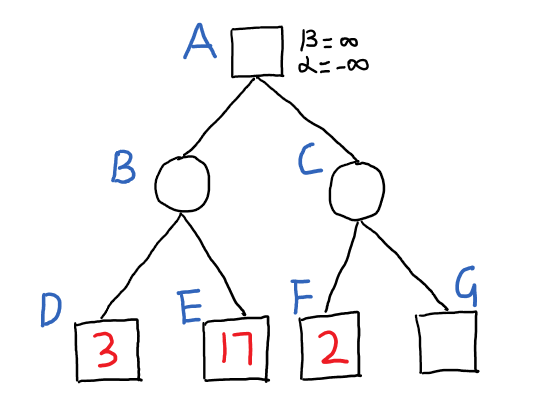
\includegraphics[scale=0.5]{assets/abt.png}
    \caption{alpha-beta剪枝示意图\label{fig:abt}} 
    \end{center} 
\end{figure} 

如\autoref{fig:abt}所示,方块结点是取最大值的结点,圆形结点是取最小值的结点。
在搜索到D时,更新$\alpha_D = 3$。在搜索到E时,更新$\alpha_E = 17$。 
回溯到结点B,它是取最小值结点,B的取值为3,更新$\beta_B = 3$。回溯到A结点
,其为最大值结点,更新A的值为3,更新$\alpha_A = 3$ 。\\

在结点A,$\alpha_A=3$,意味着可接受区间为[3, $\infty$]。即AI可以确保,
局面至少会获得$\alpha_A = 3$分。\\

在搜索到结点F时,更新$\alpha_F = 2$。回溯到结点C时,更新$\beta_C = 2$。
由于C继承了A结点的$\alpha$值,有$\alpha_C = \alpha_A = 3$。在结点C 出现了
$\alpha_C > \beta_C$,满足剪枝条件,不再对C作进一步的搜索,直接回溯到上层
结点A。\\

结点C发生的剪枝可以这样理解。AI已经能确保能获得估值为3的状态。由于结点C搜索
到了估值为2的F结点,如果AI走向C结点,玩家必然会使局势走向F结点
(或比F更差的结点)。故C结点没有进一步探索的必要了。

\section{算法伪代码}
\subsection{Minimax算法}
minimax算法的伪代码如\autoref{alg:minimax}所示。其中对Minimax函数的
调用方法见第\ref{alg:line:callminimax}行。数字8表示调用最大深度。
\begin{algorithm}
\caption{Minimax算法伪代码}
\label{alg:minimax}
\begin{algorithmic}[2]
    \Function{minimax}{node, depth, isMax}
        \If {depth == 0}
            \State \Return {evaluation}
            \Comment{返回结点的估值}
        \EndIf
        \If {isMax}
            \Comment{如果是取最大值的结点}
            \State {v $\gets -\infty$}
            \For {Each child of node}
                \State {val $\gets$ \Call{minimax}{child, depth - 1, ! isMax}}
                \State {v $\gets$ \Call{max}{v, val}}
            \EndFor
        \Else
            \Comment{如果是取最小值的结点}
            \State {v $\gets \infty$}
            \For {Each child of node}
                \State {val $\gets$ \Call{minimax}{child, depth - 1, ! isMax}}
                \State {v $\gets$ \Call{min}{v, val}}
            \EndFor
        \EndIf
        \State \Return v
    \EndFunction
    \State {}
    \State \Call {minimax}{root, 8, True}\label{alg:line:callminimax}
\end{algorithmic}
\end{algorithm}

\subsection{Alpha-beta剪枝算法}
Alpha-beta算法的伪代码见\autoref{alg:abtrunc}。其中调用方法见
\ref{alg:line:callabtrunc}行。\\

与\autoref{alg:minimax}相比,多出来的地方是,在取最大值的结点更新$\alpha$,
在取最小值的结点更新$\beta$。在$\alpha > \beta$时剪枝。
\begin{algorithm}
\caption{Alpha-beta算法伪代码}
\label{alg:abtrunc}
\begin{algorithmic}[2]
    \Function{alphabeta}{node, alpha, beta, depth, isMax}
        \If {depth == 0}
            \State \Return {evaluation}
            \Comment{返回结点的估值}
        \EndIf
        \If {isMax}
            \Comment{如果是取最大值的结点}
            \State {v $\gets -\infty$}
            \For {Each child of node}
                \State {val $\gets$ \Call{minimax}{child, alpha, beta, depth - 1, ! isMax}}
                \State {v $\gets$ \Call{max}{v, val}}
                \State {$\alpha \gets$ \Call{max}{$\alpha$, val}}
                \Comment{更新$\alpha$}
                \If {$\alpha > \beta$}
                    \State {\textbf{break}}
                \EndIf
            \EndFor
        \Else
            \Comment{如果是取最小值的结点}
            \State {v $\gets \infty$}
            \For {Each child of node}
                \State {val $\gets$ \Call{minimax}{child, alpha, beta, depth - 1, ! isMax}}
                \State {v $\gets$ \Call{min}{v, val}}
                \State {$\beta \gets$ \Call{min}{$\beta$, val}}
                \Comment{更新$\beta$}
                \If {$\alpha > \beta$}
                    \State {\textbf{break}}
                \EndIf
            \EndFor
        \EndIf
        \State \Return v
    \EndFunction
    \State {}
    \State \Call {alphabeta}{root, $-\infty, \infty$, 8, True}\label{alg:line:callabtrunc}
\end{algorithmic}
\end{algorithm}

\section{尝试的估值函数}
\subsection{数子法}
数子法的思路很简单,棋盘的估值等于己方棋子数减去对方棋子数。
\subsection{不动点估值}
不动点指的是不可能再被对方翻转的棋子。不动点相当于棋子的根基,可以认为是绝对的地盘。\\

对不动点完整的计算比较耗费时间。这里采用近似估计的方式实现。考虑到不动点一般出现在
边缘和角落的位置,故可以在估值时给予边缘和角落更大的权重。\\

采用不动点估值时,AI会更倾向于占领四周和四角,以企图获得更多的不动点。
\subsection{行动力估值}
行动力指的是,能够落子的位置的个数。行动力约低,意味着落子的可能选择越少,
局势越容易受到对方的牵制。行动力约高,意味着改变局势的可能性越大。\\

进行行动力估值的一种方式是,用己方的行动力减去对方的行动力。另一种方式是,用
己方的行动力减去对方行动力的两倍。后者的AI更倾向于压制对方的行动力,往往会在中后期
控制整个局面。
\section{关键部分代码}
alpha-beta剪枝的C++实现见\autoref{lst:minimax}。其基本上按照伪代码的
思路完成。\\

在代码中,role是一个char类型的变量,取值有BLACK('X')或WHITE('O')两种。
ChessBox是棋盘类型,有两个成员函数。Drop用来下子并翻转。dropables返回
一个可迭代对象,表示每个可落子的点。
\subsection{alpha-beta剪枝代码}
\begin{figure}[!hbt]
\begin{itemize}
\item[] \begin{lstlisting}[style=mycpp, label=lst:minimax, caption=alpha-beta剪枝代码]
double MiniMaxSolution::__solve(const ChessBox& cb, 
    const Position& position, 
    char role, 
    double alpha, 
    double beta, 
    int depth) const {

    char otherRole = role == BLACK ? WHITE : BLACK;
    // recursive base
    if (depth >= __depth) {
        return evaluation(cb);
    }

    ChessBox new_chess_box = cb;
    new_chess_box.Drop(position.first, position.second, role);

    double pivot;
    if (depth % 2 == 0) {
        // min node
        pivot = 1e8;
    } else {
        pivot = -1e8;
    }

    vector<Position> dropables = new_chess_box.Dropable(otherRole);
    if (dropables.size() == 0) {
        return evaluation(cb);
    }
    for (const auto& p : dropables) {
        double val = __solve(new_chess_box, 
            p, otherRole, 
            alpha, beta, 
            depth + 1);
        if (depth % 2 == 0) {
            // min node, update beta
            beta = std::min(beta, val);
            pivot = std::min(pivot, val);
            if (alpha >= beta) {
                break;
            }
        } else {
            // max node, update alpha
            alpha = std::max(alpha, val);
            pivot = std::max(pivot, val);
            if (alpha >= beta) {
                break;
            }
        }
    }
    return pivot;
}

\end{lstlisting}
\end{itemize}
\end{figure}

\subsection{一些估值函数的实现}
棋盘旗子估值和限制行动力估值相结合,成为本项目主要运用的估值方法。如\autoref{lst:ape}所示。\\

代码的第一个循环用来进行棋面估值。其中每个棋子占1分,每个边上的棋子占size分。
size为棋盘的大小。\\

行动力的部分,在上述的估值完成后,加上自己的行动力,减去对方的行动力。\\
\begin{figure}[!hbt]
\begin{itemize}
\item[] \begin{lstlisting}[style=mycpp, label=lst:ape, caption=限制行动力和不动点估值算法]
double ActionPressEval::evaluate(const ChessBox& chessbox, char role) const {
    char otherRole = role == BLACK ? WHITE : BLACK;
    int size = chessbox.size();
    int eval = 0;
    // 棋盘估值和不动点估值
    for (int i = 0; i < size; ++i) {
        for (int j = 0; j < size; ++j) {
            int factor;
            if (chessbox.val(i, j) == role) {
                factor = 1;
            } else if (chessbox.val(i, j) == otherRole) {
                factor = -1;
            } else {
                factor = 0;
            } 
            eval += factor;
            if (i == 0 || j == 0) {
                eval += size * factor;
            }
            if (i == size-1 || j == size-1) {
                eval += size * factor;
            }
        }
    }
    // 限制行动力估值
    eval += chessbox.Dropable(role).size() ;
    eval -= chessbox.Dropable(otherRole).size() ;
    return eval;
}
\end{lstlisting}
\end{itemize}
\end{figure}

另外一种表现不错的估值方法是行动力估值。如\autoref{lst:ode}所示。\\

事实上,在跟随机AI(永远随机选择可落子点)的对战中,行动力估值法的表现比上述的
棋盘估值和行动力限制法效果要更好。但这不一定意味着行动力估值法的棋力真的更强。\\

原因可能是,棋盘估值法过于``聪明'',会避免走很多``容易被对手将死''的路线,但
随机AI由于过于笨,很可能走不出``将死对方''的下法。这就导致棋盘估值AI太过
``谨慎'',放弃了很多高风险但高收益的下法。所以获胜得很慢。\\

但对于纯行动力AI来说,由于在开局时,棋盘空位多,能限制对方行动力的走法很少,故
纯行动力AI在刚开局时接近于随机AI,与随机AI打成平手。在棋局发展,棋子越来越多时,
纯行动力AI开始发挥作用,让随机AI的下法越来越少。最终随机AI的下法会少到只剩下
1到2种下法,甚至出现连续无法下子的情况,最终纯行动力AI让局面翻天覆地地变化。

\begin{figure}[!hbt]
\begin{itemize}
\item[] \begin{lstlisting}[style=mycpp, label=lst:ode, caption=纯行动力估值算法]
double OnlyDroppableEval::evaluate(const ChessBox& chessbox, char role) const {
    char otherRole = role == BLACK ? WHITE : BLACK;
    int size = chessbox.size();
    int eval = 0;
    eval += chessbox.Dropable(role).size() ;
    eval -= chessbox.Dropable(otherRole).size() ;
    return eval;
}
\end{lstlisting}
\end{itemize}
\end{figure}

\section{实验结果}
在本节展示的实验结果图片中,'X'均代表玩家的子,'O'均代表AI的子。其中玩家先手。
'+'代表可落子的位置。在每一个棋盘后都会附带一个数字,这个数字代表场上
的估值(数字越高对AI越有利)。
\subsection{纯行动力AI}
纯行动力AI即估值的时候,仅仅以双方行动力来估值,而不管其他条件(例如场上棋子数和
棋子分布等)。\\

事实上,纯行动力AI在和人的对战中获得了比较好的结果。在棋局刚开始时,双方还没有展示
出优势。如\autoref{fig:ode0}所示。但很快,纯行动力AI对玩家的行动力进行了
极其大的压制,玩家出现了较长时间的``下子可选位置只有2或3个''的窘境。例如
\autoref{fig:ode1}所示。图中,玩家连续两轮只有3个可落子点,但AI的可落子点
分别为13个和12个。\\

在整个对战过程中,出现了6轮玩家无法下子,3轮玩家只有1个落子点,5轮只有2个落子点,
5轮仅有3个落子点。整个对战中,甚至玩家出现过连续3轮无法落子。最终AI大比分
赢了玩家。完整的棋谱见代码压缩文件包的/log/match1.txt。

\begin{figure}[!hbt]
\begin{minipage}{0.4\textwidth}
    \centering
    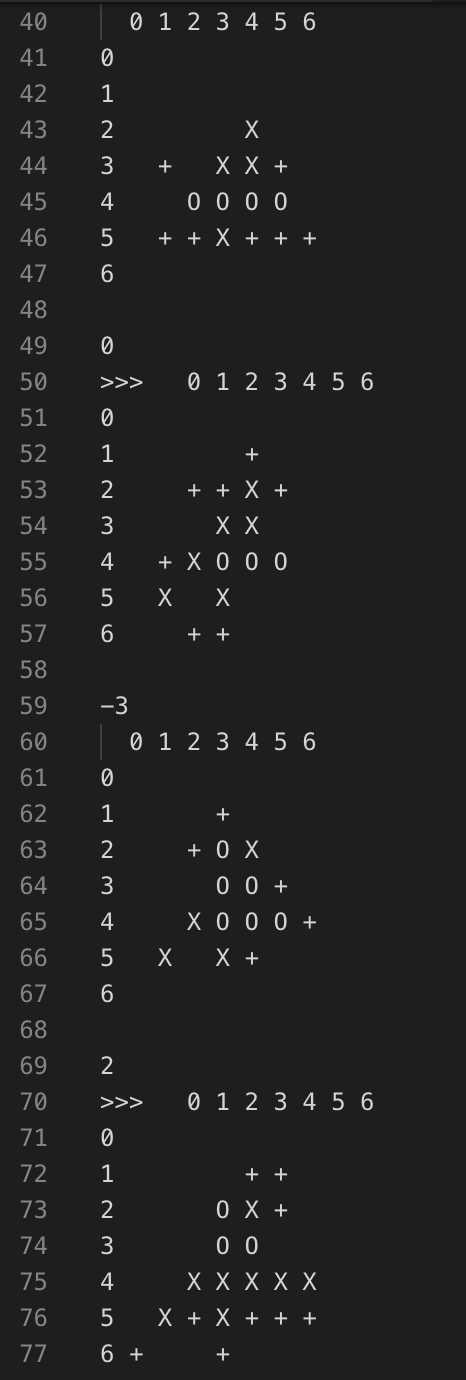
\includegraphics[width=\linewidth]{assets/ode0.png}
\caption{纯行动力AI刚开局} \label{fig:ode0}
\end{minipage}\hfill
\begin{minipage}{0.4\textwidth}
    \centering
    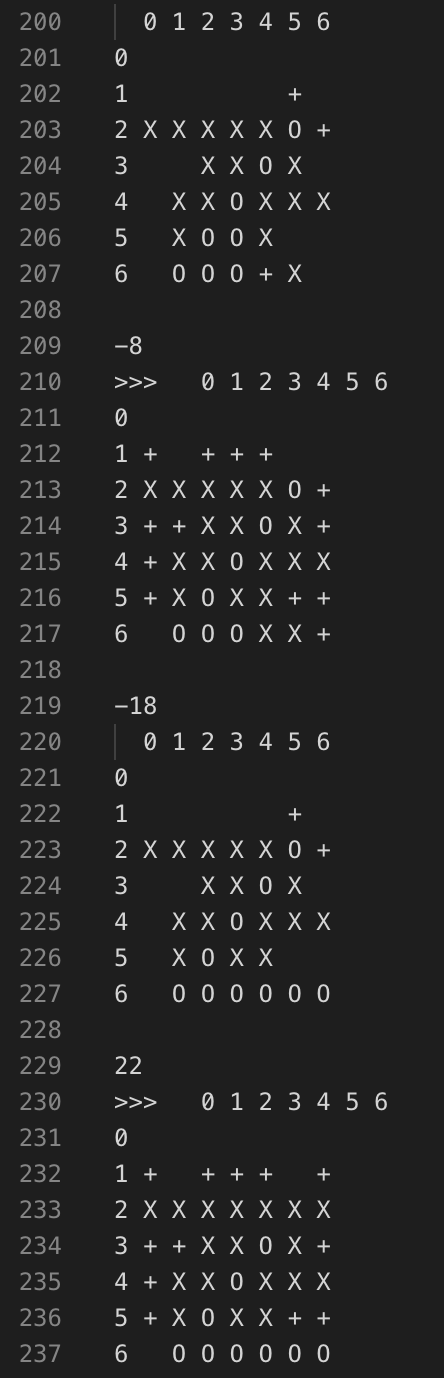
\includegraphics[width=\linewidth]{assets/ode1.png}
\caption{纯行动力AI中盘} \label{fig:ode1}
\end{minipage}
\end{figure}

\subsection{棋盘局面和行动力限制估值AI}
这个AI会综合估计场上的棋子位置进行估值,并同时参考双方的行动力进行限制。
如\autoref{fig:ape0}和\autoref{fig:ape1}所示。\\

这个AI表现得稳扎稳打。即它会与玩家来回拉锯,逐渐占据自己的有利地位。它会同时
估量自己场上的棋子数和行动力,以一定的权重考虑最优解。\\

完整的棋谱见代码压缩包中的/log/match2.txt\\

\begin{figure}[!hbt]
\begin{minipage}{0.4\textwidth}
    \centering
    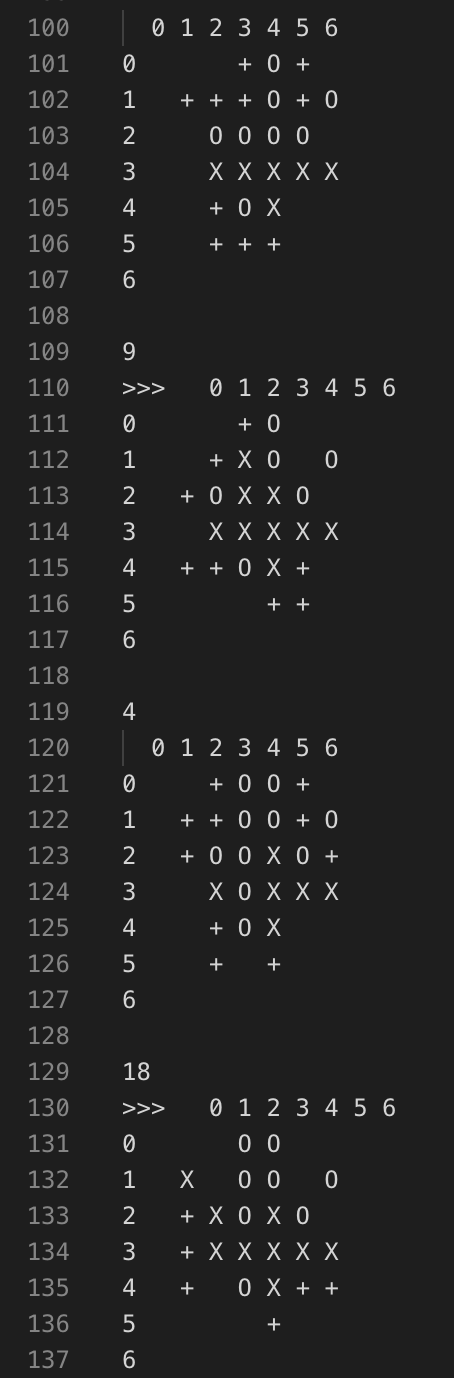
\includegraphics[width=\linewidth]{assets/ape0.png}
\caption{棋盘估值和行动力限制AI初始局面} \label{fig:ape0}
\end{minipage}\hfill
\begin{minipage}{0.4\textwidth}
    \centering
    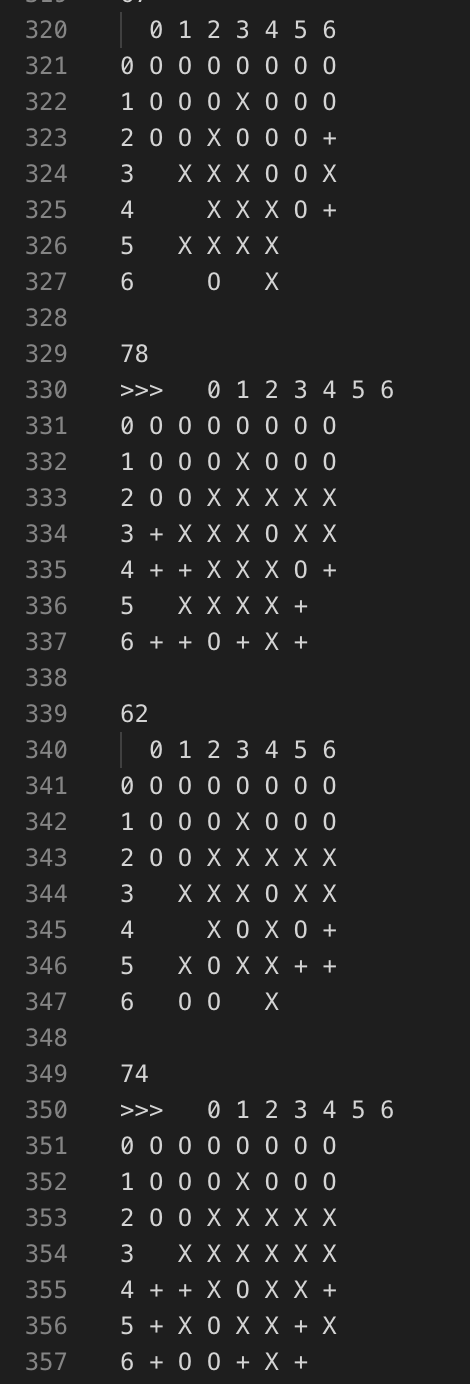
\includegraphics[width=\linewidth]{assets/ape1.png}
\caption{棋盘估值和行动力限制AI后期局面} \label{fig:ape0}
\end{minipage}
\end{figure}
\end{document}
